\documentclass[twoside]{article}
\input{ISC18-english.sty}
%%%%%%%%%%%%%%%%%%%%%%%%%%%%  Make sure to compile twice for proper cross-references. %%%%%%%%%%%%%%%%%%%%%%%
%%%%%%% For proper display of references, compile the document twice. %%%%%%%%%%%%%%%%%%%%% 
%%%%%%%%%%%%%%% If using TeX Live, compile using pdflatex command %%%%%%%%%%%%%%%%%%%%%%%
\begin{document}
\thispagestyle{empty}
%%%%%%%%%%%%%%%%% Article title header  %%%%%%%%%%%%%%%%%%%%
\fancyhead[LE]{A Similarity-based Method for Saving Runs in Factorial Experiments}
%%%%%%%%%%%%%%%%% Article authors header   %%%%%%%%%%%%%%%%%%%%
\fancyhead[RO]{Motavaze, M.}
\begin{center}
{
\includegraphics [height=25mm, width=150.3mm] {Images/isc18E}} \\
\vspace*{-1.8cm}
%\begin{center}
%\color{blue} 
%{\hspace{0.1cm}\rule{\textwidth}{1mm}}\\
%\end{center}
\vspace*{4cm}
%%%%%%%%%%%%%%%%% Article title  %%%%%%%%%%%%%%%%%%%%
{\Large \bf A Similarity-based Method for Saving Runs in Factorial Experiments }\\
%%%%%%%%%%%%%%%%% Article authors and affiliations %%%%%%%%%%%%%%%%%%%%
{\bf
Mohsen Motavaze \footnote[1]{{\bf Corresponding Author:} {\tt m.motavaze@gmail.com }}\\
%$^1$, Second Author Name   \\
$^1$ Ph.D. graduate in Statistics from the University of Isfahan, Isfahan, Iran\\
%$^2$Second Author's Affiliation
}
\end{center}
\rule{\textwidth}{0.2mm}\\
%%%%%%%%%%%%%%%%% Article abstract  %%%%%%%%%%%%%%%%%%%%
\noindent{\bf Abstract:}\\
This paper presents a method for saving experimental runs during the planning stage of factorial experiments when resources for conducting a complete experimental design are limited. In this context, the method investigates the number of coincidences between experimental runs as a measure of similarity. The real advancement of this approach lies in its emphasis on the dynamic interactions between the runs, rather than just focusing on the relationships among the factors represented as columns. Despite its simplicity, the method shows impressive performance in numerical evaluations.
 
\noindent{\bf Keywords:} 
coincidence measure, experimental run, Hamming distance, negligible contrasts, similarity. \\
\noindent{\bf Mathematics Subject Classification (2010):} $\rm 62K15$. \\
\hspace{1cm}\rule{\textwidth}{0.2mm}\\
%%%%%%%%%%%%%%
\section{Introduction}
The prevalence of missing data in practical scenarios significantly complicates model identification and misleads the statistical inference, particularly in small sample experiments (see, for example, \cite{Mot}). In many cutting-edge industrial studies, limited resources often restrict the ability to conduct complete planned experimental designs. An illustrative case is presented by \cite{Grima}, who introduced a \(2^{3}\) experiment constrained to just seven runs due to these resource limitations. This situation renders the replication of missing runs impossible, creating a clear need for a robust solution. To address this challenge, an effective estimation method is essential for balancing the demands of costly experiments with the constraints of time, materials, and budget. Several researchers have tackled this problem by employing negligible contrasts to estimate missing observations (see, \cite{Draper}, \cite{Box}, and \cite{Xampenya} amongst). Furthermore, \cite{Xampenyb} conducted a thorough analysis of which omitted runs can be estimated with desirable statistical properties. Building upon this, \cite{Grima} proposed a valuable method that defines a range of potential values for each missing result, introducing a computationally intensive simulation approach to determine which contrasts might be deemed negligible. Although their findings offer significant advancements over earlier methodologies, they can also lead to computational complexity and time delays. In light of the principles underpinning the Design of Experiments (DoE), which focus on optimizing experimentation to reduce waste while maximizing the value of collected data, we recommend a straightforward and computationally efficient method for estimating responses or saving runs under resource constraints. This approach not only aligns with the fundamental goals of DoE but also positions researchers to achieve more accurate results without compromising on resource utilization. 

The paper is organized as follows: Section \ref{sec2} presents a motivating example that illustrates the problem discussed in the subsequent sections. Section \ref{sec3} focuses on estimating missing observations when a negligible contrast is known. In Section \ref{sec4}, we introduce the similarity-based method and related concepts. Finally, Section \ref{sec5} provides a numerical evaluation to highlight the results obtained from the proposed method, along with a discussion of the designed experiment used for the evaluation.

\section{Motivation}\label{sec2}
Consider the \(2^{7-4}\) fractional factorial design in \cite{BoxH}, to investigate how seven factors, labeled A to G, influence the time it takes for a cyclist to climb a hill. The details of the experimental design and the response variable are summarized in Table \ref{tab1}. These factors pertain to both the condition of the bicycle and the cyclist. However, let's assume that one of the experimental runs could not be conducted, either due to unforeseen circumstances or limited resources. For instance, we can consider a scenario where the cyclist is unable to perform the final experimental run because of time constraints.
\begin{table}[h]
\begin{center}
\small
\caption{${2^{7-4}}$ design and the response variable.}\label{tab1}
\begin{tabular}{c|ccccccc|c}
  \hline
  run & A & B & C & D=AB & E=AC & F=BC & G=ABC & y \\
  \hline
 1& - &- &- &+ &+& + &- &69\\
2& +& -& -& -& -& + &+ &52\\
3& - &+& -& -& +& -& +& 60\\
4& +&+&-&+&-&-&-&83\\
5&-&-&+&+&-&-&+&71\\
6&+&-&+&-&+&-&-&50\\
7&-&+&+&-&-&+&-&59\\
8&+&+&+&+&+&+&+&88\\  \hline
\end{tabular}
\end{center}
\end{table}\\

\section{Negligible contrasts}\label{sec3}
Estimating missing observations in a designed experiment requires the use of estimates from runs associated with negligible a priori contrasts. This means setting the algebraic expressions of the contrasts to zero, depending on the number of missing runs (see, \cite{Box}, \cite{Xampenya}, and \cite{Grima}).
By the hierarchy principle of factorial effects and considering the value of the ABC interaction to be negligible, we can write 
\begin{equation}\label{eq1}
-y_1+y_2+y_3-y_4+y_5-y_6-y_7+y_8=0.
\end{equation}
Using the Equation (\ref{eq1}), we can estimate the missing run based on the observed values. For example, if $y_8$ represents the missing observation corresponding to the last run, we can deduce it as follows:
$$ \hat{y}_8=69-52-60+83-71+50+59=78.$$
Let $\sigma^2_y$ is the variance of the response variable. From (\ref{eq1}), $var(\hat{y}_8)=7\sigma^2_y$, and for the main effect $A$ we have 
$$A=\frac{1}{4}(-y_1+y_2-y_3+y_4-y_5+y_6-y_7+y_8),$$
and $var(A)=\frac{\sigma^2_y}{2}$. But, with an estimated run, for example $\hat{y}_8$, we have
$$A=\frac{1}{4}(-y_1+y_2-y_3+y_4-y_5+y_6-y_7+(y_1-y_2-y_3+y_4-y_5+y_6+y_7)),$$
and $var(A)={\sigma^2_y}$. 


Although the method is straightforward, it significantly inflates the variance of estimated response variable, effectively doubling the variance of the factorial effects and complicating model identification. In the next section, we aim to address this issue and estimate the missing runs.
%\subsection{Simulation-based algorithm}
%Grima et al considered the situation when it is not known that which contrasts will be negligible. The method is based on first establishing an interval of possible values corresponding to each of the missing results, then identifying which contrasts are always null independently of the value of said results.  
\section{Similarity based method}\label{sec4}
In the experiment described in Section \ref{sec2}, which consists of 7 runs and has 6 degrees of freedom, we can estimate 6 factorial effects. Following the hierarchy of effects, we focus on the main effects $A-F$. Figure \ref{fig11} illustrates the factorial plots for the effects we are considering.
\begin{figure}[h]
\begin{center}
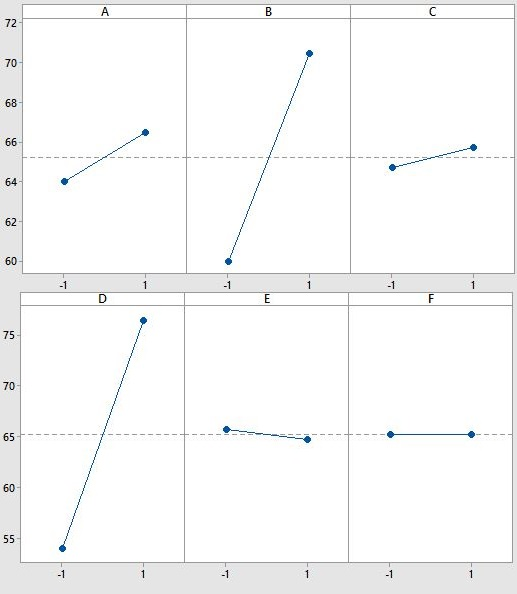
\includegraphics[width=7cm,height=6cm]{Images/abc.jpg}\\
%
\includegraphics[width=7cm,height=6cm]{Images/Fig1-eps-converted-to.pdf}\\
\vspace{-0.2cm}
\caption{\footnotesize{Factorial effects plot.}}\label{fig11}
\end{center}
\end{figure} 

According to the results shown in Figure \ref{fig11}, we can exclude factors E and F from our analysis; and project the design onto factors A, B, C, and D, treating the data as an incomplete non-replicated factorial design, as illustrated in Table \ref{tab2}.

 \begin{table}[h]
\begin{center}
\small
\caption{The projected design and the response variable.}\label{tab2}
\begin{tabular}{c|cccc|c}
  \hline
  run & A & B & C& D & y \\
  \hline
 1& - &- & -& +&69\\
2& +& -& - &-&52\\
3& - &+& -& - & 60\\
4& +&+& -&+&83\\
5&-&-& +& + &71\\
6&+&-& +& -&50\\
7&-&+& +&-&59\\
8&+&+& +&+& NA\\  \hline
\end{tabular}
\end{center}
\end{table}
%\begin{rem}\label{rm1}
%The above displays a replicated regular design. 
%\end{rem}
\subsection{Coincidence matrix}
This section introduces a robust measure of coincidence designed to quantify the similarities between different runs; which allows for a nuanced understanding of how similar or dissimilar these runs are with respect to one another. The key innovation of this approach is its emphasis on investigating the relationships between the runs, which are represented as rows in the dataset, rather than merely focusing on the relationships between the factors, represented as columns. This shift in perspective can lead to more meaningful analyses and results.%This shift in perspective not only enhances the analytical depth but also facilitates the identification of patterns that may otherwise be overlooked, leading to more informed conclusions and decisions based on the data.

 \begin{dfn}\label{df1}
For a design $D=[x_{ij}]_{N \times n}$ the number of coincidence between the $i^{th}$ and $j^{th}$ rows is 
$$\delta_{ij}(D)=\sum_{k=1}^n \delta(x_{ik},x_{jk}),$$
where $\delta(x,y)$ is the Kronecker delta function.
\end{dfn}
\begin{rem}\label{rm2}
The quantity $H_{ij}=n - \delta_{ij}(D)$ is known as the {\it Hamming distance} between the $i^{th}$ and $j^{th}$ rows in algebraic coding theory. 
\end{rem}
\begin{dfn}\label{df2}
Based on the Definition \ref{df1} for any design $D=[x_{ij}]_{N \times n}$ the coincidence matrix is defined as
\[M= 
\begin{pmatrix} 
n & \delta_{12} & ... & \delta_{1n}\\
\delta_{21}& n & ... & \delta_{2n}\\
. & . & n  & .\\
\delta_{N1}& 0 & ... & n\\
\end{pmatrix}
\]
\end{dfn}
\begin{rem}
The coincidence matrix defined above, is a symmetric matrix. 
\end{rem}
\begin{eg}\label{ex1}
For the design in Table \ref{tab2}, the coincidence matrix is
\[M= 
\begin{pmatrix} 
4 & 2 & 2 & 2 & 3 &  1 & 1 & 1\\
2 & 4 & 2 & 2 & 1 &  3 & 1 & 1\\
2 & 2 & 4 & 2 & 1 &  1 & 3 & 1\\
2 & 2 & 2 & 4 & 1 &  1 & 1 & 3\\
3 & 1 & 1 & 1 & 4 &  2 & 2 & 2\\
1 & 3 & 1 & 1 & 2 &  4 & 2 & 2\\
1 & 1 & 3 & 1 & 2 &  2 & 4 & 2\\
1 & 1 & 1 & 3 & 2 &  2 & 2 & 4\\
\end{pmatrix}
\]
\end{eg} 

\subsection{Grouping the runs}
The coincidence matrix is utilized to group runs based on their similar distance values. Larger values indicate greater similarity between the runs. Therefore, the following grouping is recommended for the number of runs.
\begin{equation}\label{eqg}
\mathcal{G}_1=\lbrace 1, 5 \rbrace, \mathcal{G}_2=\lbrace 2, 6 \rbrace, \mathcal{G}_3=\lbrace 3, 7 \rbrace, \mathcal{G}_4=\lbrace 4, 8 \rbrace. 
\end{equation}
Therefore, if $y_8$ is the missing run, we have
$\hat{y}_8=y_4,$
and from the grouping in (\ref{eqg}), $var(\hat{y}_8)=\sigma^2_y$. Therefore, the effects will have the same variance as if all runs had been conducted; and $var(A)=\frac{\sigma^2_y}{2}$. 

\section{Numerical evaluation}\label{sec5}
To effectively illustrate the advantages of the similarity-based method over the negligible contrast method, we conducted a numerical comparison of missing observations. In a randomized run order, any experimental run could end up being the last one, which might prevent the cyclist from completing it. Table \ref{tab3} clearly presents the differences between our innovative approach and the traditional method that treats negligible contrasts as zero when estimating missing runs. This numerical analysis compellingly showcases the superiority of our method in effectively addressing the challenges posed by missing data, as well as, improvement in terms of variance estimates.
\begin{table}[h]
\begin{center}
\small
\caption{The observations and their estimated values.}\label{tab3}
\begin{tabular}{c|cccccccc}
  \hline
run   & 1 & 2 & 3& 4 & 5 & 6 & 7 &8 \\
  \hline
 observed response variable & 69 & 52 & 60 & 83 & 71 & 50 & 59 &88\\
  \hline
      estimated value by negligible contrasts & 79 & 42 & 50 & 93 &61& 60 & 69 & 78\\
\hline
estimated value by the proposed method & 71 & 50 & 59 & 88 &69& 52 & 60 & 83\\
  \hline
\end{tabular}
\end{center}
\end{table}
%%%%%%%%%%%%%%%%%%%%%%% Definition %%%%%%%%%%%%%%%%%%%%%%%%%%%%%%%%%%%

%%%%%%%%%%%%%%%%%%%%%%% Example %%%%%%%%%%%%%%%%%%%%%%%%%%%%%%%%%%%

%%%%%%%%%%%%%%%%%%%%%%% Lemma %%%%%%%%%%%%%%%%%%%%%%%%%%%%%%%%%%%
%\begin{lem}\label{lm1}
%This is a lemma.
%\end{lem}
%%%%%%%%%%%%%%%%%%%%%%% Theorem and proof  %%%%%%%%%%%%%%%%%%%%%%%%%%%%%%%%%%%
%\begin{thm}\label{th1}
%This is a theorem.
%\end{thm}
%\begin{proof}
%This is a proof. 
%\end{proof}
%%%%%%%%%%%%%%%%%%%%%%%  Proposition  %%%%%%%%%%%%%%%%%%%%%%%%%%%%%%%%%%%
%\begin{pro}\label{pr1}
%This is a proposition.
%\end{pro}
%%%%%%%%%%%%%%%%%%%%%%% Corollary %%%%%%%%%%%%%%%%%%%%%%%%%%%%%%%%%%%
%\begin{cor}\label{cor1}
%This is a corollary.
%\end{cor}
%%%%%%%%%%%%%%%%%%%%%%% Remark %%%%%%%%%%%%%%%%%%%%%%%%%%%%%%%%%%%
%\begin{rem}\label{rm1}
%You can refer to definition \ref{df1}, lemma \ref{lm1}, theorem \ref{th1}, proposition \ref{pr1}, and
%corollary \ref{cor1} in the text.
%\end{rem}
%%%%%%%%%%%%%%%%%%%%%%% Algorithm %%%%%%%%%%%%%%%%%%%%%%%%%%%%%%%%%%%
%\begin{alg}\label{alg1}
%This algorithm has the following \footnote{Steps}steps:
%\begin{itemize}
%\item 
%Step 1
%\item
%Step 2
%\item
%Step 3
%\end{itemize}
%\end{alg}
%\section{Formulas}
%%%%%%%%%%%%%%%%%%%%%%%%%%%%%%% Unnumbered formula %%%%%%%%%%%%%%%%%%%%%%%
%A sample unnumbered formula is given below:
%\begin{equation*}
%\max\limits_{x \in \mathbb{R}} \ f(x).
%\end{equation*}
%%%%%%%%%%%%%%%%%%%%%%%%%%%%%%% Numbered formula %%%%%%%%%%%%%%%%%%%%%%%
%Here is a sample of a numbered formula: 
%\begin{equation}\label{eq11}
%G_F(x)=\frac{1}{B(\alpha,\beta)}\int_{0}^{F(x)} t^{\alpha-1}(1-t)^{\beta-1}\,dt, \qquad \alpha>0, \beta>0.
%\end{equation}
%Formula numbering should be based on sections, and only relationships that are referenced in the text should have numbers.
%Below is a multiline formula that is the derivative of equation \eqref{eq1}:
%\begin{align}
%g_F(x)&=\frac{d}{dx} G_F(x)\nonumber\\
%&=\frac{1}{B(\alpha,\beta)} f(x) \left(F(x)\right)^{\alpha -1} \left(\bar F(x)\right)^{\beta -1}.
%\end{align}
%\section{Tables and Figures}
%Below is a sample table. Table \ref{tab1} contains four rows and three columns.
%\begin{table}[h]
%\begin{center}
%\small
%\caption{Table title should be here.}\label{tab1}
%\begin{tabular}{|c|cc|}
  %\hline
  %Column One & Column Two & Column Three \\  \hline \hline
  %1 & 2 & 3 \\
  %4 & 5 & 6 \\
  %7 & 8 & 9 \\  \hline
%\end{tabular}
%\end{center}
%\end{table}\\
%%%%%%%%%%%%%%%%%%%%%%%%%%%%%%% Figure %%%%%%%%%%%%%%%%%%%%%%%%%%%%%%%%%
%Below is a sample figure. Figure \ref{fig1} contains two subfigures.
%\begin{figure}[ht]
%\begin{center}
%
\includegraphics[width=7cm,height=6cm]{Images/Fig2-eps-converted-to.pdf}
%
\includegraphics[width=7cm,height=6cm]{Images/Fig1-eps-converted-to.pdf}\\
%\vspace{-0.2cm}
%\caption{\footnotesize{Figure caption should be placed here.}}\label{fig1}
%\end{center}
%\end{figure}
%\section{How to Cite References}
%References must be cited in the text. \cite{Craik:2005}, \cite{Feller:1972}, \cite{Genest:Rivest:1993}, and \cite{LZ15} are some examples of English references.
\section*{Discussion and Conclusion}   
This paper introduces an innovative method that leverages the relationships among runs (i.e., rows) instead of focusing solely on factors (i.e., columns). By identifying similar runs, we can effectively substitute their corresponding response values when faced with missing observations, ensuring more accurate and reliable outcomes.
%\section*{Acknowledgments}   
%If you wish to include acknowledgments, this section should appear before the references.
%%%%%%%%%%%%%%%%%%%%%%%% References %%%%%%%%%%%%%%%%%%%%%%%%%%%%%

\begin{thebibliography}{9}
\bibitem[Box (1990)]{Box}
Box, G.E.P. 1990. A simple way to deal with missing observations from DOE , {\it Quality Engineering } 3(2):249-254.

\bibitem[Box et al (2005)]{BoxH}
Box, G.E.P., Hunter, J.S., Hunter, W.G. 2005. {\it Statistics for experimenters: design, innovation, and discovery },
Hoboken: Wiley.

\bibitem[Draper and Stoneman (1964)]{Draper}
Draper, N., Stoneman, D. 1964. Estimating missing values in unreplicated two-level factorial and fractional factorial designs, {\it Biometrics } 20(3):443-458.

\bibitem[Grima et al (2019)]{Grima}
Grima, P., Rodero, L., & Tort-Martorell, X. 2019. Saving runs in fractional factorial designs, {\it Quality Engineering } 31(3):375-385.

%\bibitem[Feller (1972)]{Feller:1972} 
%Feller W. (1972), {\it An introduction to probability theory and its applications,} New York, John Wiley.

%\bibitem[Genest and  Rivest (1993)]{Genest:Rivest:1993}
%Genest C. and  Rivest L.P. (1993), Statistical inference
%procedures for bivariate Archimedean copulas, {\it J. Amer.
%Statist. Assoc.} 88,  1034 - 1043.
\bibitem[Motavaze and Talebi (2023)]{Mot}
Motavaze, M., & Talebi, H. 2023. Design criteria for model discrimination in factorial experiments with potential failing runs, {\it Stat } 12(1):e536.

%\bibitem[Li et al. (2015)]{LZ15}
%Li K., Zheng W. and Ai M. (2015), Optimal designs for the proportional interference model, {\it The Annals of Statistics}, 43(4), 1596-1616.
\bibitem[Xampeny et al (2017)]{Xampenya}
Xampeny, R., Grima, P. and Tort-Martorell, X. 2017. Estimating missing values from negligible interactions in factorial designs, {\it Quality and Reliability Engineering International}, 33(6):1235-1247.

\bibitem[Xampeny et al (2018)]{Xampenyb}
Xampeny, R., Grima, P. and Tort-Martorell, X. 2018. Which runs to skip in two-level factorial designs when not all can be performed, {\it Quality Engineering}, Published Online: 4 Apr 2018  .

\end{thebibliography}
 \end{document}

